\documentclass[12pt]{extarticle}
\usepackage{tempora}
\usepackage[T1, T2A]{fontenc}
\usepackage[utf8]{inputenc}
\usepackage[english, ukrainian]{babel}
\usepackage{geometry}
\usepackage{graphicx}
\usepackage{multirow}
\usepackage{multicol}
\usepackage{float}
\graphicspath{{/home/artem/Pictures}}
\geometry
{
    a4paper,
    left=30mm,
    top=15mm,
    right=20mm,
    bottom=15mm,
}

\begin{document}
\begin{titlepage}
    \begin{center}
        \textbf{\normalsize{\MakeUppercase{
            Міністерство Освіти і науки України
            Національний університет "Львівська політехніка"
        }}}

        \begin{flushright}
        \textbf{ІКНІ}\\
        Кафедра \textbf{ПЗ}
        \end{flushright}
        \vspace{15mm}

        \includegraphics[width=0.4\textwidth]{lpnu_logo.png}

        \vspace*{\fill}

        \textbf{\normalsize{\MakeUppercase{Звіт}}}
            
        До лабораторної роботи №5

        \textbf{на тему:} “ Метод сортування підрахунком.”

        \textbf{з дисципліни:} "Алгоритми і структури даних”
            
        \vspace*{\fill}

        \begin{flushright}

            \textbf{Лектор:}\\
            доцент кафедри ПЗ\\
            Коротєєва Т. О.\\
            \vspace{12pt}

            \textbf{Виконав:}\\
            студент групи ПЗ-24\\
            Губик А. С.\\
            \vspace{12pt}

            \textbf{Прийняв:}\\
            асистент кафедри ПЗ\\
            Вишневський К. О.\\
        \vspace{12pt}
        \end{flushright}

        Львів -- 2023
            
            
    \end{center}
\end{titlepage}

\subsection*{Тема роботи} 
Метод сортування підрахунком.

\subsection*{Мета роботи} Вивчити алгоритм сортування підрахунком. Здійснити програмну реалізацію алгоритму сортування підрахунком. Дослідити швидкодію алгоритму сортування підрахунком.

\subsection*{Індивідуальне завдання}
До кожного елемента застосувати $x^2$



\subsection*{Теоретичні відомості}
Сортування підрахунком (англійською «Counting Sort») — алгоритм впорядкування, що застосовується при малій кількості різних елементів (ключів) у масиві даних. Час його роботи лінійно залежить як від загальної кількості елементів у масиві так і від кількості різних елементів.

Ідея алгоритму полягає в наступному: спочатку підрахувати скільки разів кожен елемент (ключ) зустрічається в вихідному масиві. Спираючись на ці дані можна одразу вирахувати на якому місці має стояти кожен елемент, а потім за один прохід поставити всі елементи на свої місця.

В алгоритмі присутні тільки прості цикли довжини N (довжина масиву), та один цикл довжини K (величина діапазону). Отже, обчислювальна складність роботи алгоритму становить O(N + K).

В алгоритмі використовується додатковий масив. Тому алгоритм потребує E(K) додаткової пам’яті.

В такій реалізації алгоритм є стабільним. Саме ця його властивість дозволяє використовувати його як частину інших алгоритмів сортування (наприклад, сортування за розрядами).

Використання даного алгоритму є доцільним тільки у випадку малих K.


\subsection*{Покроковий опис}

\begin{enumerate}

\item \textbf{Функція:} До кожного елемента застосовуємо $x^2$
\item \textbf{Ініціалізація:} По-перше, ініціалізуємо два додаткові масиви 
- один для підрахунку кількості входжень кожного елемента та інший для 
зберігання відсортованих елементів.
\item \textbf{Знаходження діапазону:} Знаходимо мінімальний та максимальний 
елементи у вихідному масиві, щоб визначити діапазон значень.
\item \textbf{Підрахунок кількості входжень:} Створюємо масив count, де індекси
 відповідають унікальним елементам в діапазоні, і для кожного 
 елемента підраховуємо кількість його входжень в вхідний масив.
  Тобто, count[i] буде містити кількість елементів зі значенням i.
\item \textbf{Суми кількостей:} За допомогою масиву count розраховуємо кількості елементів, які менші або рівні кожному унікальному значенню. Це визначає позицію, на яку буде поміщено кожний елемент у відсортованому масиві.
\item \textbf{Побудова відсортованого масиву:} Проходимо вхідний масив зліва направо і визначаємо позицію кожного елемента у відсортованому масиві, використовуючи масив count. Після цього зменшуємо значення count для відповідного елемента.
\item \textbf{Отримання відсортованого масиву:} На цьому етапі маємо відсортований масив зі збереженими елементами в правильному порядку.


\end{enumerate}

\subsection*{Вихідний код}

{\fontfamily{pcr}\selectfont
\begin{verbatim}
#include <iostream>
#include <vector>
#include <cstdlib>
#include <ctime>
#include <algorithm>
#include <chrono>

// Counting Sort function
void countingSort(std::vector<int>& arr) {
    int maxElement = *std::max_element(arr.begin(), arr.end());
    int minElement = *std::min_element(arr.begin(), arr.end());
    int range = maxElement - minElement + 1;

    std::vector<int> count(range);
    std::vector<int> output(arr.size());

    for (int i = 0; i < arr.size(); i++) {
        count[arr[i] - minElement]++;
    }

    for (int i = 0; i < range; i++) {
        std::cout << count[i];
    }
    std::cout << '\n';

    for (int i = 1; i < range; i++) {
        count[i] += count[i - 1];
    }

    for (int i = arr.size() - 1; i >= 0; i--) {
        output[count[arr[i] - minElement] - 1] = arr[i];
        count[arr[i] - minElement]--;
    }

    for (int i = 0; i < range; i++) {
        std::cout << count[i];
    }
    std::cout << '\n';

    for (int i = 0; i < arr.size(); i++) {
        arr[i] = output[i];
    }
}

int main() {
    // Seed the random number generator
    std::srand(static_cast<unsigned>(std::time(nullptr)));

    // Get the size of the vector from the user
    int vectorSize;
    std::cout << "Enter the size of the vector: ";
    std::cin >> vectorSize;

    // Generate a vector of random integers within a specified range
    std::vector<int> numbers;
    int minRange = -100;  // Minimum range value
    int maxRange = 100;   // Maximum range value

    for (int i = 0; i < vectorSize; i++) {
        int randomInt = std::rand() % (maxRange - minRange + 1) + minRange;
        numbers.push_back(randomInt);
    }

    // Measure sorting time
    auto startTime = std::chrono::high_resolution_clock::now();

    // Counting Sort the vector
    countingSort(numbers);

    auto endTime = std::chrono::high_resolution_clock::now();
    auto duration = std::chrono::duration_cast<std::chrono::nanoseconds>(endTime - startTime);

    // Print the sorted vector
    std::cout << "Sorted Vector:" << std::endl;
    for (const int& num : numbers) {
        std::cout << num << " ";
    }
    std::cout << std::endl;

    std::cout << "Sorting time: " << duration.count() << " nanoseconds" << std::endl;

    return 0;
}

\end{verbatim}
}
\vspace{12pt}
\begin{figure}[H]
    \centering
    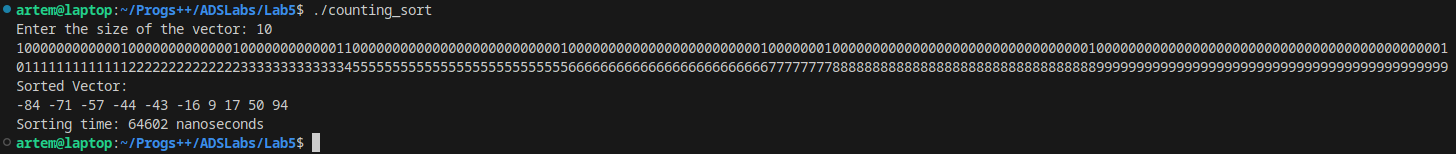
\includegraphics[width=0.90\textwidth]{Screenshot_20231018_010132.png}
    \caption{}
\end{figure}
\subsection*{Висновок} 
Сортування підрахунком є ефективним, коли діапазон можливих 
значень досить обмежений, але воно не вимагає порівнянь між
 елементами, що робить його швидким алгоритмом сортування.
\end{document}
